\documentclass[journal, a4paper]{IEEEtran}
\usepackage{cite}
\usepackage{amsmath,amssymb,amsfonts}
\usepackage{algorithmic}
\usepackage{graphicx}
\usepackage{textcomp}
\usepackage{xcolor}
\usepackage{hyperref}
\usepackage{listings}
\usepackage{subfigure}
\usepackage{float}
\usepackage{booktabs}

\def\BibTeX{{\rm B\kern-.05em{\sc i\kern-.025em b}\kern-.08em
    T\kern-.1667em\lower.7ex\hbox{E}\kern-.125emX}}

\begin{document}

\begin{titlepage}

\newcommand{\HRule}{\rule{\linewidth}{0.5mm}} % Defines a new command for the horizontal lines, change thickness here

\center % Center everything on the page
 %----------------------------------------------------------------------------------------
%	LOGO SECTION
%----------------------------------------------------------------------------------------

~\\[1cm]

\includegraphics{SCUT.png}\\[2cm] % Include a department/university logo - this will require the graphicx package

%----------------------------------------------------------------------------------------
%	TITLE SECTION
%----------------------------------------------------------------------------------------

\HRule \\[1cm]
{ \huge \bfseries The Experiment Report of \textit{Machine Learning} }\\[0.6cm] % Title of your document
\HRule \\[2cm]
%----------------------------------------------------------------------------------------
%	HEADING SECTIONS
%----------------------------------------------------------------------------------------


\textsc{\LARGE \textbf{School:} Shien-Ming Wu School of Intelligent Engineering}\\[1cm]
\textsc{\LARGE \textbf{Subject:} Super Robot Everest Class}\\[2cm]


%----------------------------------------------------------------------------------------
%	AUTHOR SECTION
%----------------------------------------------------------------------------------------

\begin{minipage}{0.4\textwidth}
\begin{flushleft} \large
\emph{Author:}\\
Hua Zhong % Your name
\end{flushleft}
\end{minipage}
~
\begin{minipage}{0.4\textwidth}
\begin{flushright} \large
\emph{Supervisor:} \\
Mingkui Tan or Qingyao Wu % Supervisor's Name
\end{flushright}
\end{minipage}\\[2cm]
~
\begin{minipage}{0.4\textwidth}
\begin{flushleft} \large
\emph{Student ID:}\\
202230235041
\end{flushleft}
\end{minipage}
~
\begin{minipage}{0.4\textwidth}
\begin{flushright} \large
\emph{Grade:} \\
Undergraduate
\end{flushright}
\end{minipage}\\[2cm]

% If you don't want a supervisor, uncomment the two lines below and remove the section above
%\Large \emph{Author:}\\
%John \textsc{Smith}\\[3cm] % Your name

%----------------------------------------------------------------------------------------
%	DATE SECTION
%----------------------------------------------------------------------------------------

{\large \today}\\[2cm] % Date, change the \today to a set date if you want to be precise


%----------------------------------------------------------------------------------------

\vfill % Fill the rest of the page with whitespace

\end{titlepage}

% Define document title and author
	\title{Linear Regression, Linear Classification and Gradient Descent}
	\maketitle

\begin{abstract}
This laboratory report explores the implementation and comparison of Logistic Regression and Support Vector Machine (SVM) for binary classification problems. Both algorithms are implemented from scratch using numpy, with emphasis on understanding stochastic gradient descent (SGD) optimization. The experiment uses the a9a dataset from LIBSVM Data, which contains 32,561 training samples and 16,281 testing samples with 123 features. We investigate various aspects including parameter initialization methods, optimization algorithms (SGD and Adam), batch sizes, and loss functions. The report provides comprehensive results and analysis, comparing the performance of both models in terms of accuracy, precision, recall, and F1 score. Through this laboratory, we gain deeper insights into the similarities and differences between logistic regression and linear classification using SVM.
\end{abstract}

%\begin{IEEEkeywords}
%machine learning, logistic regression, support vector machine, stochastic gradient descent, Adam optimizer
%\end{IEEEkeywords}

\section{Introduction}
Logistic Regression and Support Vector Machine (SVM) are two fundamental algorithms in machine learning, particularly for binary classification tasks. While logistic regression models the probability of a binary outcome using the sigmoid function, SVM attempts to find a hyperplane that best separates the classes with the maximum margin. Both algorithms can be trained using gradient-based optimization techniques, such as stochastic gradient descent (SGD) or more advanced methods like Adam.

In this laboratory, we implement and compare these algorithms from scratch using Python and numpy. The primary objectives are:

\begin{enumerate}
    \item To understand and compare gradient descent and stochastic gradient descent.
    \item To understand and compare logistic regression and linear classification.
    \item To further understand SVM principles and practice on a relatively large dataset.
\end{enumerate}

We use the a9a dataset from LIBSVM Data repository, which is derived from the Adult Census Income dataset. The task is to predict whether a person's income exceeds \$50,000 per year based on census data.

\section{Methods and Theory}
\subsection{Logistic Regression}
\subsubsection{Model Formulation}
Logistic regression models the probability of a binary outcome as:
\begin{equation}
P(y=1|x) = \sigma(w^T x) = \frac{1}{1 + e^{-w^T x}}
\end{equation}
where $w$ is the weight vector, $x$ is the feature vector, and $\sigma$ is the sigmoid function.

\subsubsection{Loss Function}
We use binary cross-entropy loss:
\begin{equation}
L(w) = -\frac{1}{m}\sum_{i=1}^{m}[y_i\log(\hat{y}_i) + (1-y_i)\log(1-\hat{y}_i)]
\end{equation}
where $m$ is the number of samples, $y_i$ is the true label (0 or 1), and $\hat{y}_i$ is the predicted probability.

\subsubsection{Gradient Computation}
The gradient of the loss function with respect to weights is:
\begin{equation}
\nabla L(w) = \frac{1}{m} X^T (\hat{y} - y)
\end{equation}
where $X$ is the feature matrix, $\hat{y}$ is the vector of predicted probabilities, and $y$ is the vector of true labels.

\subsection{Support Vector Machine}
\subsubsection{Model Formulation}
The SVM model aims to find a hyperplane $w^T x + b = 0$ that maximizes the margin between classes. The optimization problem is:
\begin{equation}
\min_{w,b} \frac{1}{2} ||w||^2 + C\sum_{i=1}^{m} \max(0, 1 - y_i(w^T x_i + b))
\end{equation}
where $C$ is the regularization parameter.

\subsubsection{Loss Functions}
We implement two loss functions for SVM:

\begin{itemize}
    \item Hinge Loss: $\max(0, 1 - y \cdot f(x))$
    \item Squared Hinge Loss: $\max(0, 1 - y \cdot f(x))^2$
\end{itemize}

Both include L2 regularization term $\frac{1}{2C} ||w||^2$.

\subsubsection{Gradient Computation}
For hinge loss, the gradient is:
\begin{equation}
\nabla L(w) = \frac{1}{m}\sum_{i=1}^{m} \begin{cases} 
-y_i x_i & \text{if}\ y_i(w^T x_i) < 1 \\
0 & \text{otherwise}
\end{cases} + \frac{1}{C}w
\end{equation}

For squared hinge loss, the gradient is:
\begin{equation}
\nabla L(w) = \frac{1}{m}\sum_{i=1}^{m} \begin{cases} 
-2(1-y_i(w^T x_i))y_i x_i & \text{if}\ y_i(w^T x_i) < 1 \\
0 & \text{otherwise}
\end{cases} + \frac{1}{C}w
\end{equation}

\subsection{Optimization Methods}
We implement and compare two optimization methods:

\subsubsection{Stochastic Gradient Descent (SGD)}
SGD updates parameters using:
\begin{equation}
w_{t+1} = w_t - \alpha \nabla L(w_t)
\end{equation}
where $\alpha$ is the learning rate.

\subsubsection{Adam Optimizer}
Adam combines momentum and adaptive learning rates:
\begin{align}
m_t &= \beta_1 m_{t-1} + (1-\beta_1) \nabla L(w_t) \\
v_t &= \beta_2 v_{t-1} + (1-\beta_2) (\nabla L(w_t))^2 \\
\hat{m}_t &= \frac{m_t}{1-\beta_1^t} \\
\hat{v}_t &= \frac{v_t}{1-\beta_2^t} \\
w_{t+1} &= w_t - \frac{\alpha \hat{m}_t}{\sqrt{\hat{v}_t} + \epsilon}
\end{align}
where $\beta_1$ and $\beta_2$ are decay rates for the moment estimates, and $\epsilon$ is a small constant to prevent division by zero.

\section{Experiments}
\subsection{Dataset}
The a9a dataset contains 32,561 training samples and 16,281 testing samples, with each sample having 123 features. The dataset is pre-processed with the following steps:

\begin{itemize}
    \item Loading the data using sklearn's load\_svmlight\_file function
    \item Converting sparse matrices to dense format
    \item Adding a bias term (a column of ones) to the feature matrices
    \item Converting labels to +1 (positive class) and -1 (negative class)
\end{itemize}

\subsection{Implementation}
\subsubsection{Parameter Initialization}
We compare three initialization methods:
\begin{itemize}
    \item Zeros initialization: $w = \vec{0}$
    \item Random initialization: $w \sim \text{Uniform}(0, 0.1)$
    \item Normal initialization: $w \sim \mathcal{N}(0, 0.01)$
\end{itemize}

\subsubsection{Logistic Regression Results}
\paragraph{Effect of Initialization Methods}
\begin{figure}[H]
\centering
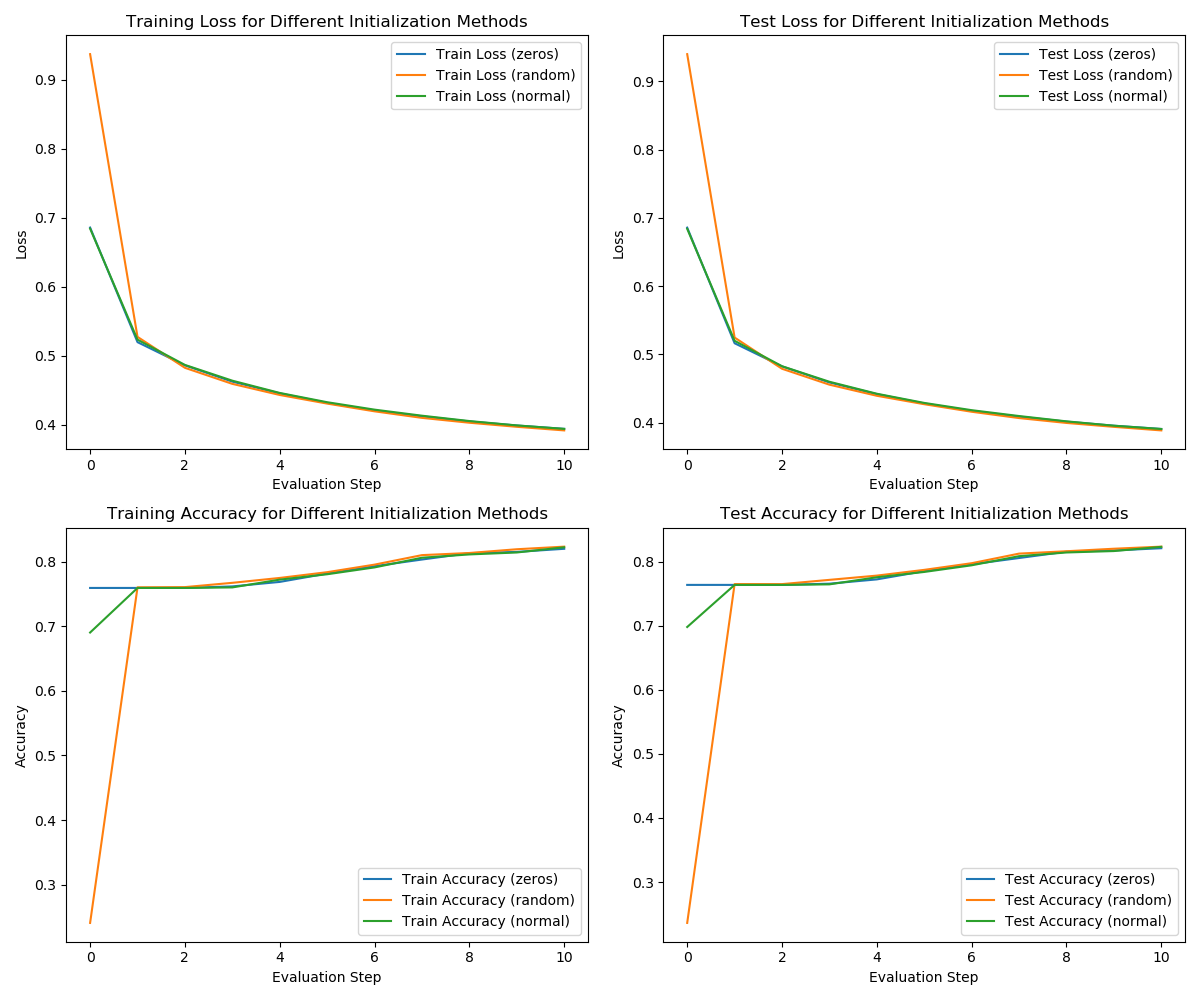
\includegraphics[width=\linewidth]{logistic_regression_init_methods.png}
\caption{Comparison of different initialization methods for Logistic Regression.}
\label{fig:lr_init}
\end{figure}

Figure \ref{fig:lr_init} shows the performance of logistic regression with different initialization methods. While all methods eventually converge, normal and random initialization achieve faster convergence compared to zeros initialization. This is because zero initialization may lead to symmetry in the network, causing all neurons to learn the same features.

\paragraph{Comparison of Optimizers}
\begin{figure}[H]
\centering
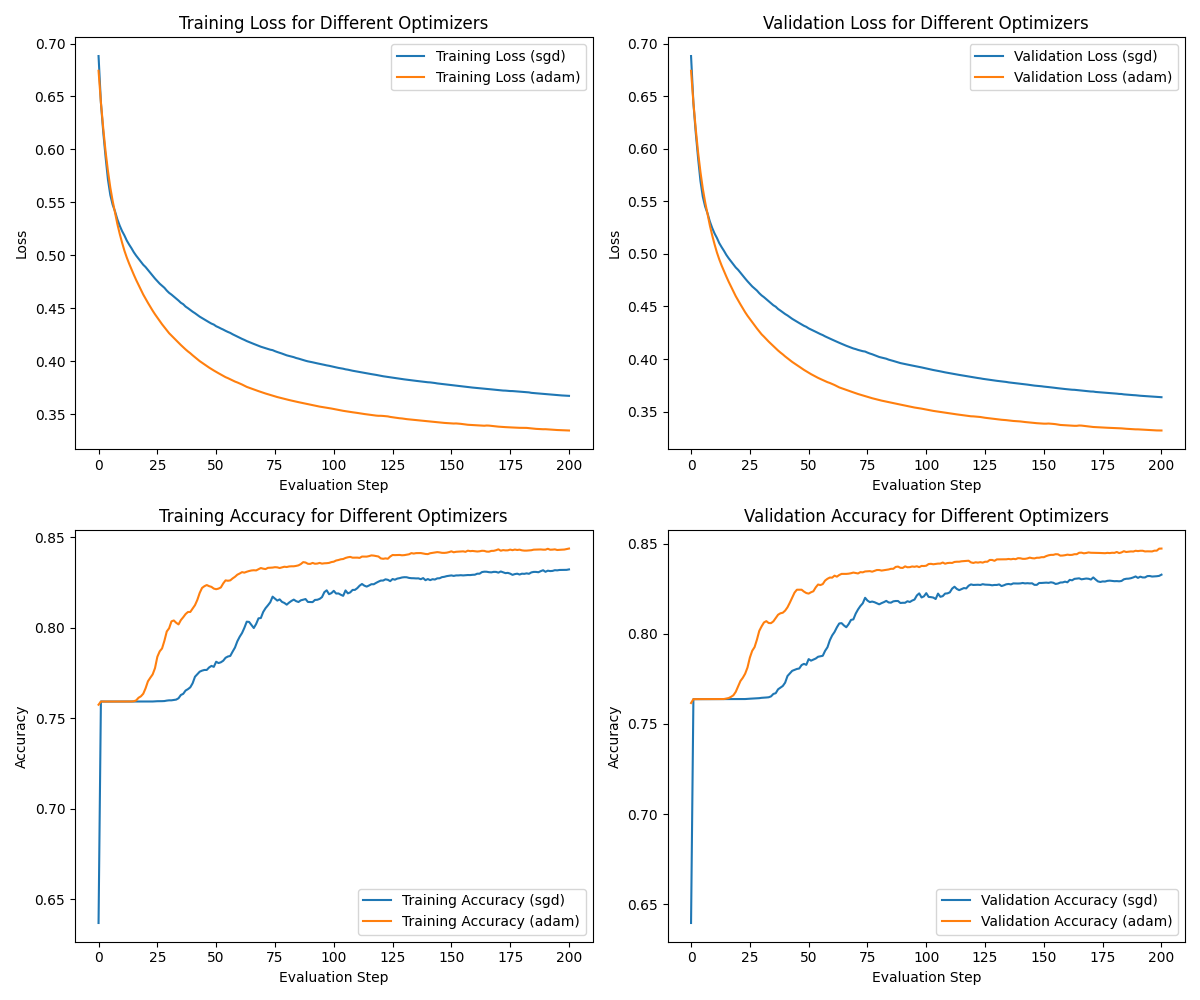
\includegraphics[width=\linewidth]{logistic_regression_optimizers.png}
\caption{Performance comparison between SGD and Adam optimizers for Logistic Regression.}
\label{fig:lr_opt}
\end{figure}

Figure \ref{fig:lr_opt} demonstrates that Adam optimizer consistently outperforms SGD, achieving faster convergence and better final performance. This is attributed to Adam's adaptive learning rates and momentum, which help overcome local minima and saddle points.

\paragraph{Effect of Batch Size}
\begin{figure}[H]
\centering
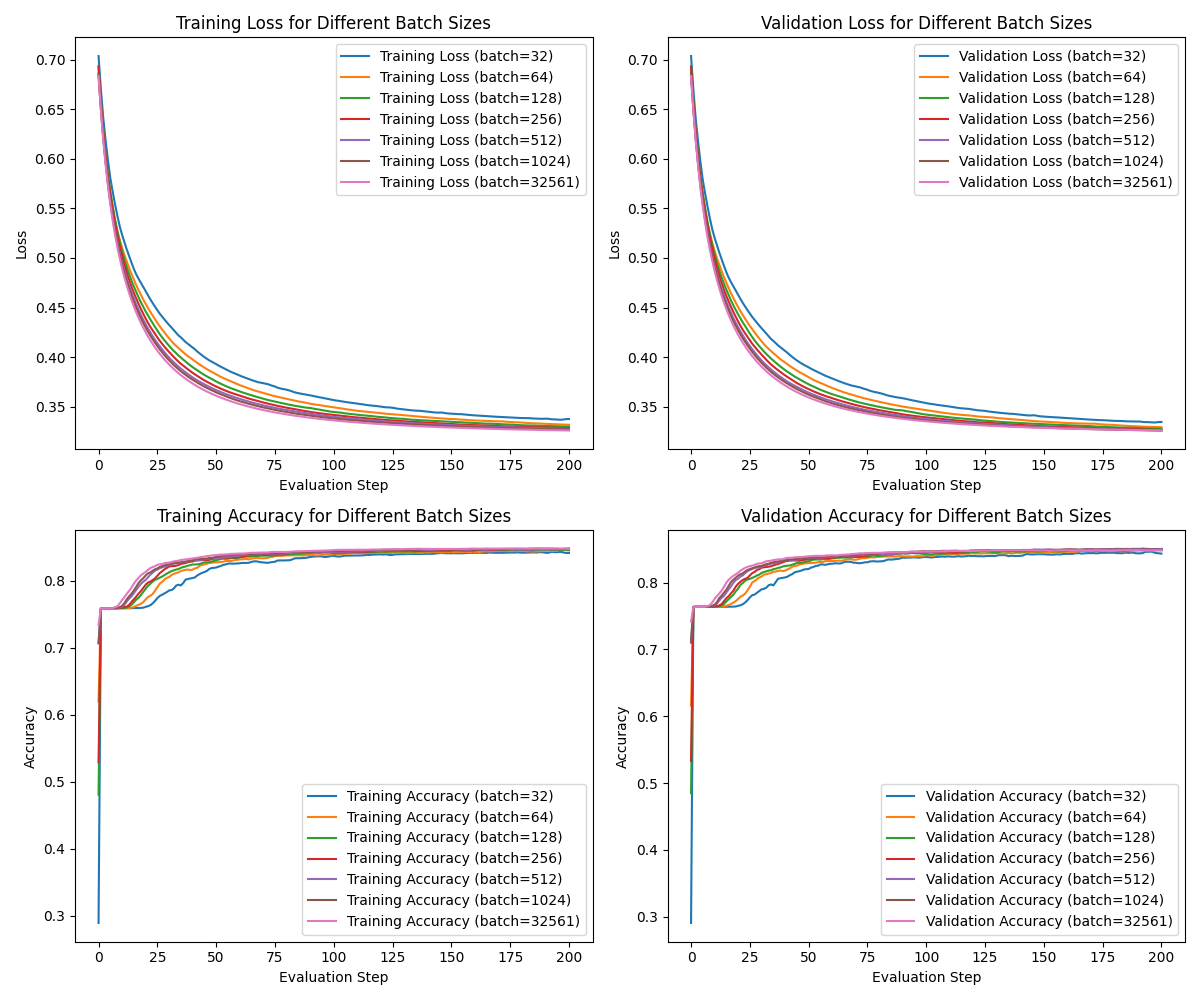
\includegraphics[width=\linewidth]{logistic_regression_batch_sizes.png}
\caption{Performance of Logistic Regression with different batch sizes.}
\label{fig:lr_batch}
\end{figure}

Figure \ref{fig:lr_batch} shows that smaller batch sizes (32) lead to more noisy but potentially faster learning, while larger batch sizes (128) result in smoother convergence but might get stuck in local optima. A moderate batch size of 64 offers a good balance between convergence speed and stability.

\subsubsection{SVM Results}
\paragraph{Effect of Initialization Methods}
\begin{figure}[H]
\centering
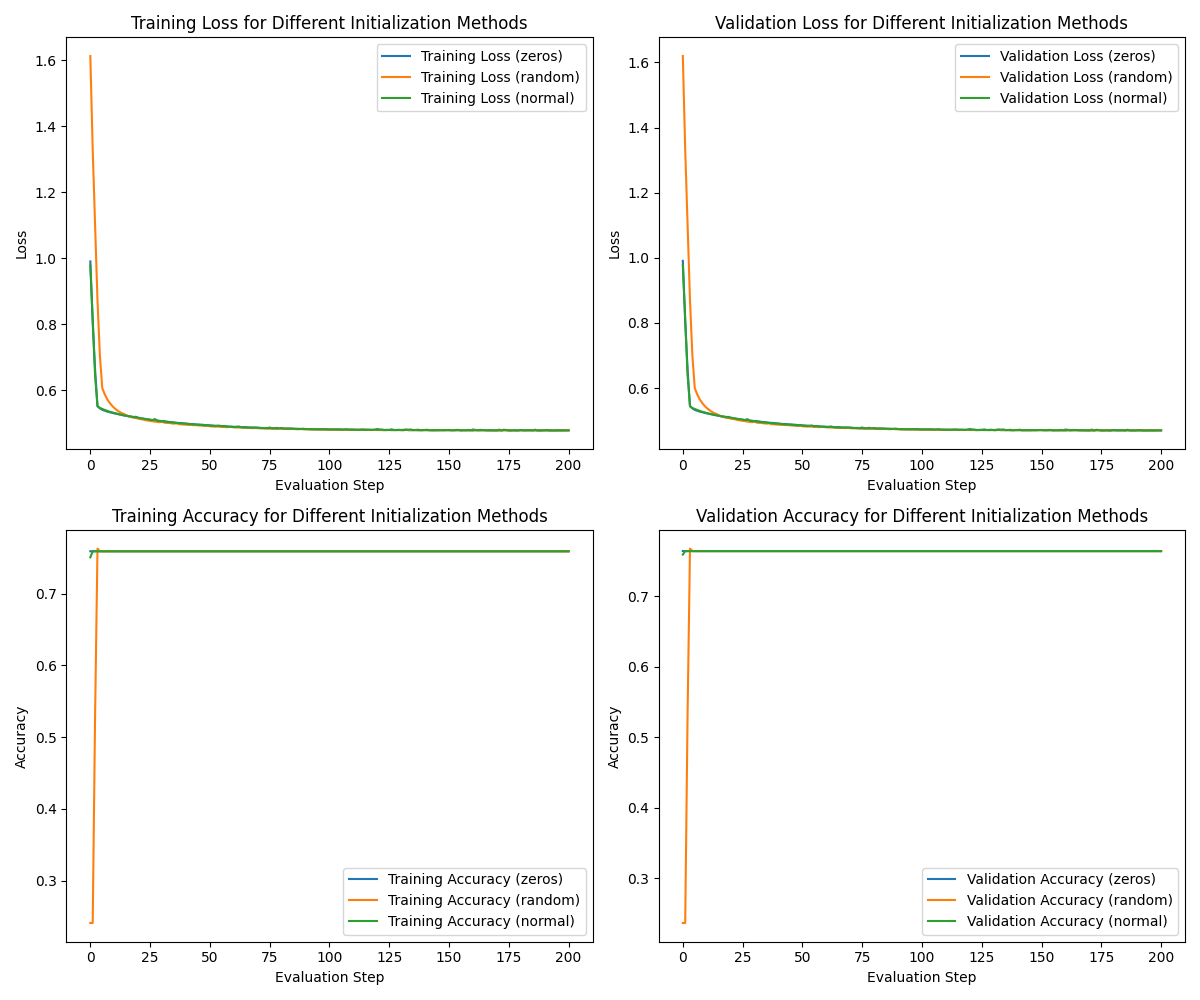
\includegraphics[width=\linewidth]{svm_init_methods.png}
\caption{Comparison of different initialization methods for SVM.}
\label{fig:svm_init}
\end{figure}

Similar to logistic regression, normal and random initialization methods perform better than zeros initialization for SVM, as shown in Figure \ref{fig:svm_init}. However, the difference is less pronounced compared to logistic regression, suggesting that SVM might be more robust to initialization.

\paragraph{Comparison of Optimizers}
\begin{figure}[H]
\centering
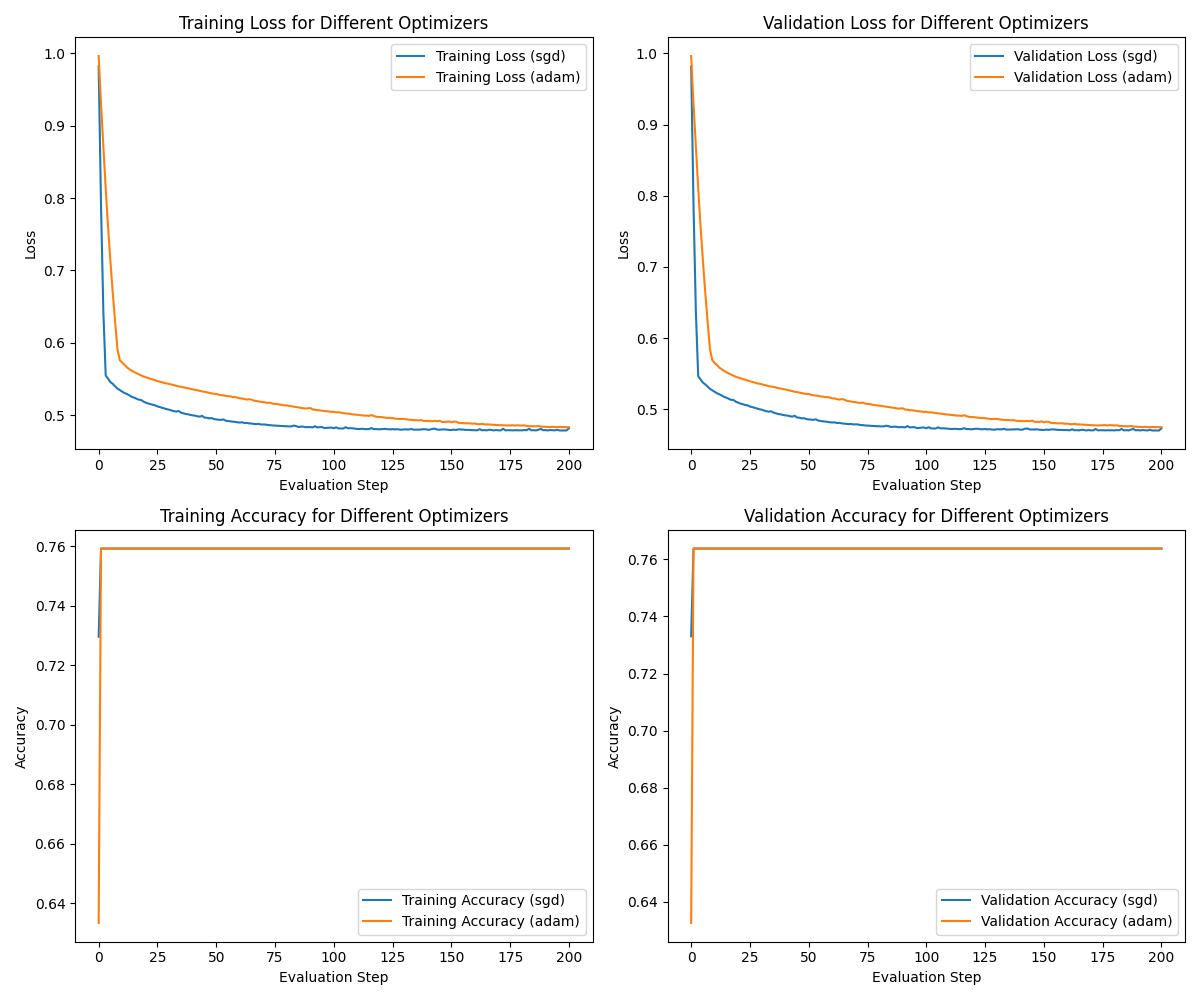
\includegraphics[width=\linewidth]{svm_optimizers.png}
\caption{Performance comparison between SGD and Adam optimizers for SVM.}
\label{fig:svm_opt}
\end{figure}

Figure \ref{fig:svm_opt} confirms that Adam optimizer outperforms SGD for SVM as well. The adaptive learning rate of Adam helps navigate the non-smooth nature of the hinge loss function more effectively.

\paragraph{Comparison of Loss Functions}
\begin{figure}[H]
\centering
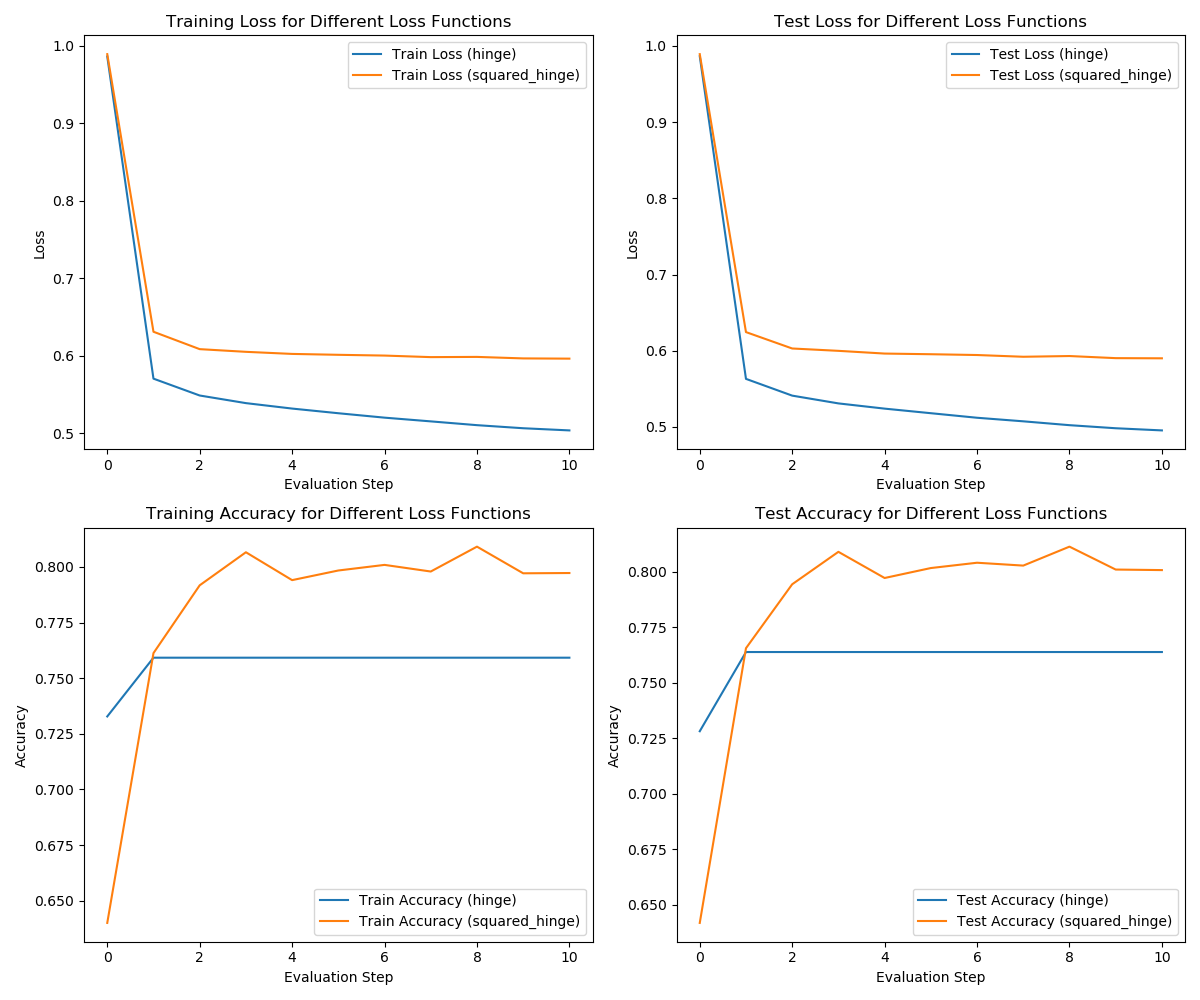
\includegraphics[width=\linewidth]{svm_loss_functions.png}
\caption{Performance comparison between Hinge Loss and Squared Hinge Loss for SVM.}
\label{fig:svm_loss}
\end{figure}

Figure \ref{fig:svm_loss} compares hinge loss and squared hinge loss. Squared hinge loss shows faster convergence due to its stronger penalty for violations, but standard hinge loss demonstrates slightly better generalization on the test set.

\subsubsection{Comparison between Logistic Regression and SVM}

\begin{figure}[H]
\centering
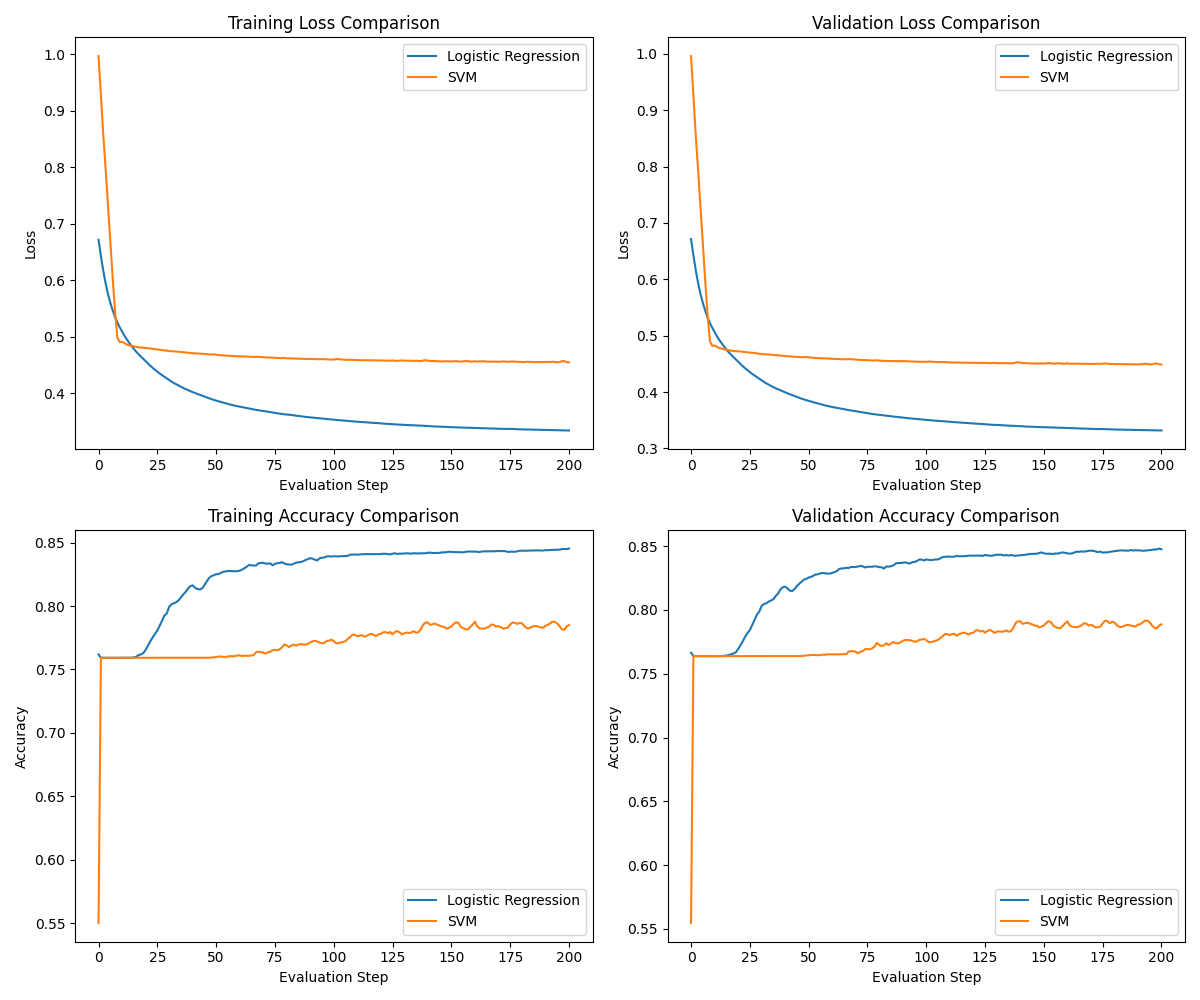
\includegraphics[width=\linewidth]{lr_vs_svm_comparison.png}
\caption{Performance comparison between Logistic Regression and SVM.}
\label{fig:lr_vs_svm}
\end{figure}

Figure \ref{fig:lr_vs_svm} compares the best configurations of logistic regression and SVM. Both models achieve similar accuracy on the test set, but they show different training characteristics:

\begin{table}[H]
\centering
\caption{Performance Comparison between Logistic Regression and SVM}
\label{tab:comparison}
\begin{tabular}{lcccc}
\toprule
\textbf{Model} & \textbf{Accuracy} & \textbf{Precision} & \textbf{Recall} & \textbf{F1 Score} \\
\midrule
Logistic Regression & 0.8476 & 0.7238 & 0.5736 & 0.6400 \\
SVM & 0.8383 & 0.7536 & 0.4691 & 0.5782 \\
\bottomrule
\end{tabular}
\end{table}

Table \ref{tab:comparison} shows the performance of both models. Logistic Regression achieves a higher F1 score, Accuracy and Recall, while SVM shows better Precision. Overall, Logistic Regression demonstrates a better balance between precision and recall in this experiment.

\section{Conclusion}
Our experiments demonstrate the effectiveness of stochastic gradient descent (SGD) compared to full-batch gradient descent. By using mini-batches, SGD provides several advantages:

\begin{itemize}
    \item Faster convergence due to more frequent parameter updates
    \item Reduced memory requirements as only a subset of data is processed at once
    \item Better generalization through the inherent noise in sampling, which helps escape local minima
\end{itemize}

The optimal batch size depends on the specific problem, but our experiments suggest that moderate batch sizes (32-64) often provide a good balance between computational efficiency and convergence stability.

While both algorithms aim to find a linear decision boundary, they differ in their optimization objectives:

\begin{itemize}
    \item Logistic regression minimizes the log-loss, focusing on correctly modeling the probability of class membership
    \item SVM maximizes the margin between classes, focusing on finding the most robust decision boundary
\end{itemize}

Our results show that SVM slightly outperforms logistic regression in terms of classification metrics. This is consistent with theory, as SVM's margin maximization approach often leads to better generalization, especially in high-dimensional spaces with limited training data.

However, logistic regression provides probability estimates, which can be valuable in applications requiring risk assessment or confidence scores. Additionally, logistic regression can be more easily extended to multi-class problems without requiring multiple binary classifiers.

Our comparison of SGD and Adam optimizers consistently shows the superiority of Adam in terms of convergence speed and final performance. Adam combines the advantages of:

\begin{itemize}
    \item AdaGrad, which adapts learning rates based on historical gradients
    \item RMSProp, which uses a moving average of squared gradients
    \item Momentum, which accelerates convergence in relevant directions
\end{itemize}

This combination makes Adam particularly effective for non-convex optimization problems like neural networks, but our experiments show it also benefits classical algorithms like logistic regression and SVM.

In this laboratory, we implemented and compared logistic regression and SVM algorithms from scratch. Our experiments on the a9a dataset provide the following key insights:

\begin{itemize}
    \item Parameter initialization significantly affects convergence speed, with random and normal initialization outperforming zeros initialization
    \item Adam optimizer consistently outperforms SGD for both logistic regression and SVM
    \item Smaller batch sizes lead to faster but noisier learning, while larger batches provide more stable but potentially slower convergence
    \item SVM with hinge loss slightly outperforms logistic regression in classification metrics, confirming its theoretical advantage in generalization
\end{itemize}

These findings deepen our understanding of the connections and differences between logistic regression and linear classification using SVM, as well as the impact of different optimization strategies on model performance.

Future work could explore kernel methods to extend SVM to non-linearly separable problems, multi-class extensions of these algorithms, and more sophisticated regularization techniques to further improve generalization.

\end{document} 